\documentclass{article}
\usepackage[utf8]{inputenc}
\usepackage{indentfirst}
\usepackage[nottoc,notlot,notlof]{tocbibind}
\usepackage{url}
\usepackage{hyperref}
\usepackage{listings}
\usepackage[export]{adjustbox}

\begin{document}
\thispagestyle{empty}
\begin{center}
{\large Master 1 - Ingénierie Informatique} \\ [0.5cm]
\vfill
\rule{\linewidth}{0.4mm} \\ [0.4cm]
{\huge \bfseries
Travaux d'Etude et de Recherche\\
- \\
GraphoScan \\ [0.4cm]
Mémoire Final \\ [0.4cm]
}
\rule{\linewidth}{0.4mm} \\ [1.5cm]

\begin{minipage}{0.4\textwidth}
\begin{flushleft} \large
Thibault \textsc{Charpignon} \\
Benoît \textsc{Gallet} \\
Emmanuel \textsc{Herrmann} \\
Martin \textsc{Réty}
\end{flushleft}
\end{minipage}

\vfill

\large\emph{Encadré par : }{Matthieu \textsc{Exbrayat}}

\vfill


{\large 6 Février - 22 Mai 2017}

\end{center}

\newpage
\setcounter{page}{1}
\tableofcontents

\newpage

\section{Résumé du projet}

\subsection{Présentation}

Ce projet de TER prolonge un travail déjà entamé l'année dernière par deux étudiants de Polytech, consistant à enregistrer en vidéo l'écriture d'un calligraphe, pour pouvoir reconstruire un modèle en 3D du mouvement de la plume. Une structure en bois supporte deux caméras, que l'on peut bouger le long de rails puis fixer à l'aide de vis. Le calligraphe écrit sous cette structure et la feuille est éclairée par des spots lumineux. Il faut alors associer l'image des deux caméras, ce qui n'est pas possible nativement avec le logiciel fourni par le fabricant (FlyCapture de PointGrey) pour faire de l'acquisition vidéo en stéréo, puis reconstituer via OpenGL les mouvements de la plume. Ces mouvements ont été sauvegardés grâce à des algorithmes de tracking, travaillant sur les vidéos enregistrées auparavant.



\subsection{But du projet}

Ce projet permettra à terme de réaliser une reconstitution 3D des mouvements du calligraphe. On pourra alors lui faire recopier plusieurs textes, provenant de différents lieux et différentes époques, afin de pouvoir comparer les styles d'écriture, définir s'il existait différentes écoles d'écriture, différents styles, etc. De manière plus générale, le projet pourra servir pour beaucoup d'applications par la suite, car le code final se voudra le plus généraliste possible.

\section{Analyse de l'existant}

\subsection{Fonctionnement de l'application}

Cette section présente le fonctionnement global de l'application, afin de mieux cerner le sujet sur lequel nous avons travaillé. Il faut cependant préciser que ce n'est pas sous cette forme que nous avons reçu le projet, il ne fonctionnait que partiellement, la version présentée ici est la version finale post-TER.

\begin{figure}[!h]
\centering
\includegraphics[scale=0.08]{Modules/Picture/Utilisation.png}
\caption{Ecriture et acquisition}
\label{utilisation}
\end{figure}

Le dispositif montré sur la figure \ref{utilisation} nous permet de capturer les vidéos en direct. Ces deux vidéos sont enregistrées sur ordinateur, pour pouvoir faire de la stéréo : on encode les images en même temps pour avoir exactement les mêmes frames au même moment. On applique ensuite des paramètres d'undistortion pour lisser les bords de l'image. En effet, la caméra ayant un grand angle, l'extérieur de l'image est déformé, ce qui peut apporter des problèmes lors de la reconstruction 3D.

Une fois les deux vidéos récupérées, on peut lancer la reconstruction. La première étape est de retrouver l'écriture sur l'image, pour cela différentes méthodes sont disponibles. On peut par exemple faire du tracking. Après avoir sélectionné une zone d'intérêt grâce à un ROI (Region Of Interest) selector (figure \ref{ROI} ), on essaye de suivre le mouvement. Il suffit d'enregistrer les coordonnées du centre du point pour retrouver le mouvement dessiné (figure \ref{tracking} ).

La seconde technique est celle du HOG (Histogramme de gradient orienté) qui permet de détecter des formes dans une image. Ce qui donne au départ une image comme sur la figure \ref{HOGSale}, et après nettoyage \ref{HOGPropre}.

L'une ou l'autre de ces techniques peuvent être utilisées pour avoir une suite de coordonnées correspondant au dessin de l'écriture. Une fois que ces deux coordonnées sont récupérées, il existe des fonctions dans OpenCV pour faire des points 3D à partir de points 2D. Il faut pour cela récupérer les paramètres extrinsèques (matrices de rotation et vecteurs de translation, pour passer du repère lié à l'espace de travail au repère lié à la caméra) de la caméra.

Une fois que les coordonnées sont récupérées par l'une ou l'autre méthode, une fonction nous permet de rajouter deux points entre chaque coordonnée pour fluidifier la ligne. Ces coordonnées sont ensuite interprétées par OpenGL pour permettre de les afficher dans un repère en trois dimensions (figures \ref{3D1} et \ref{3D2} ).


\begin{figure}[htb]
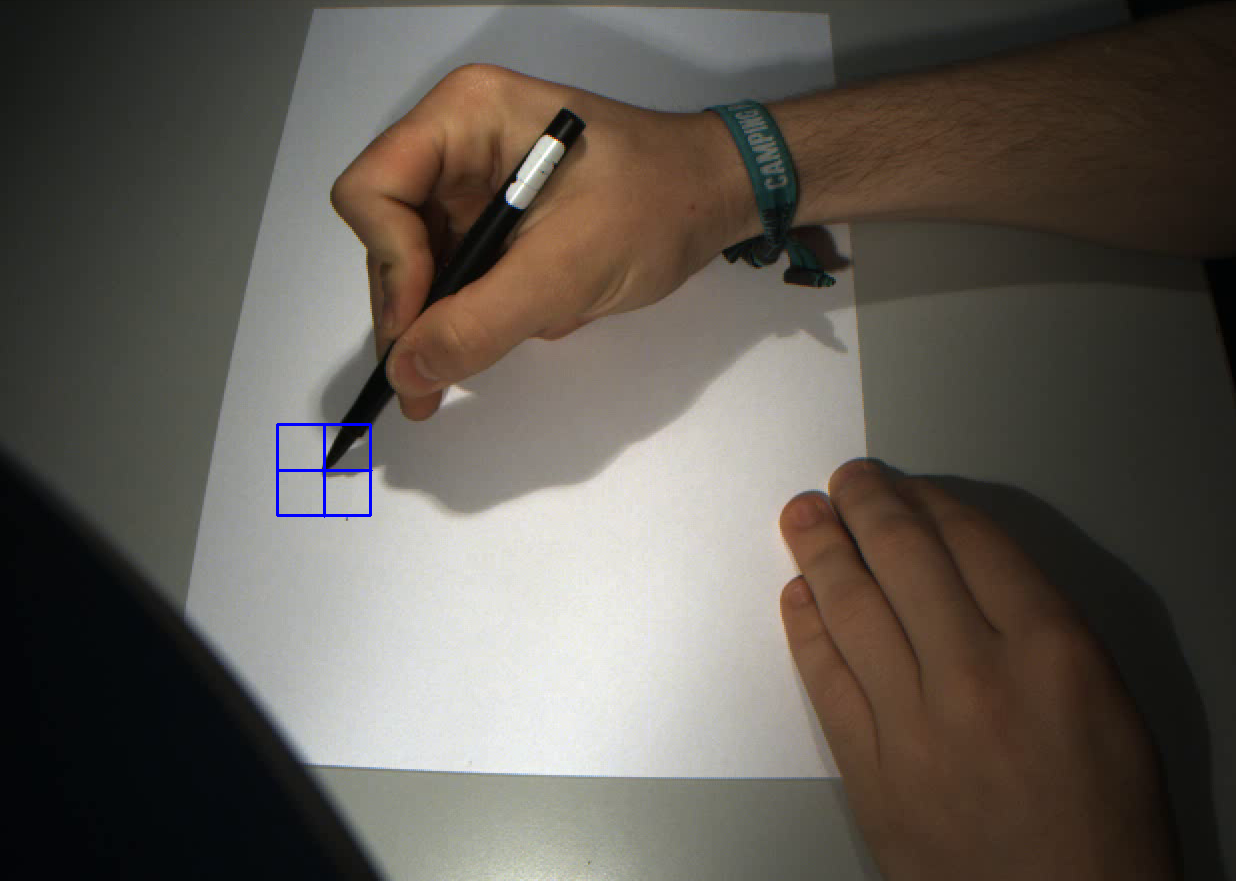
\includegraphics[width=\textwidth]{Modules/Picture/roi}
\caption{ROI selector}
\label{ROI}
\vspace{30px}
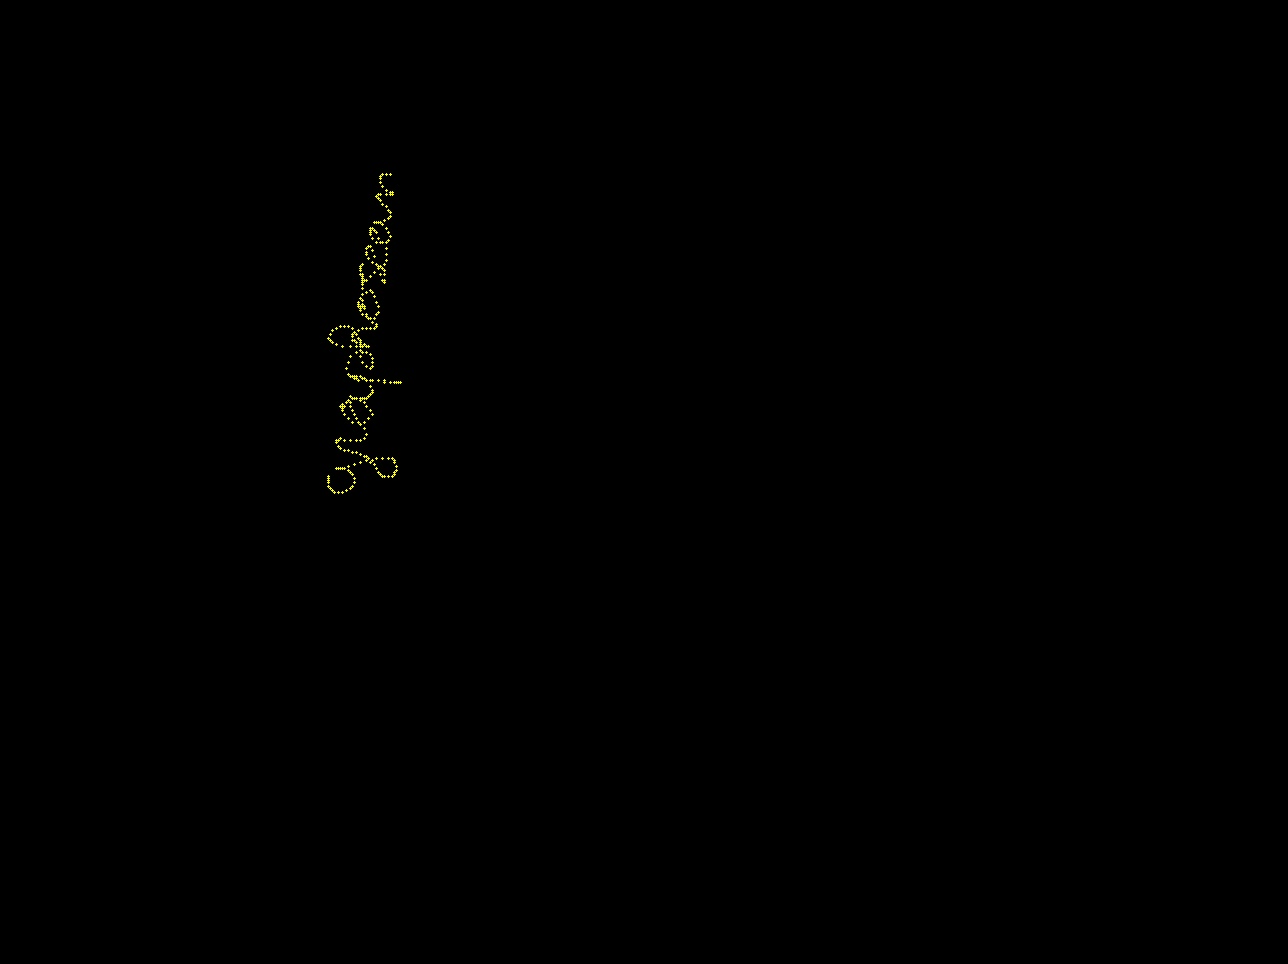
\includegraphics[width=\textwidth]{Modules/Picture/tracking}
\caption{Reconnaissance avec le tracking}
\label{tracking}
\end{figure}

\newpage

\begin{figure}
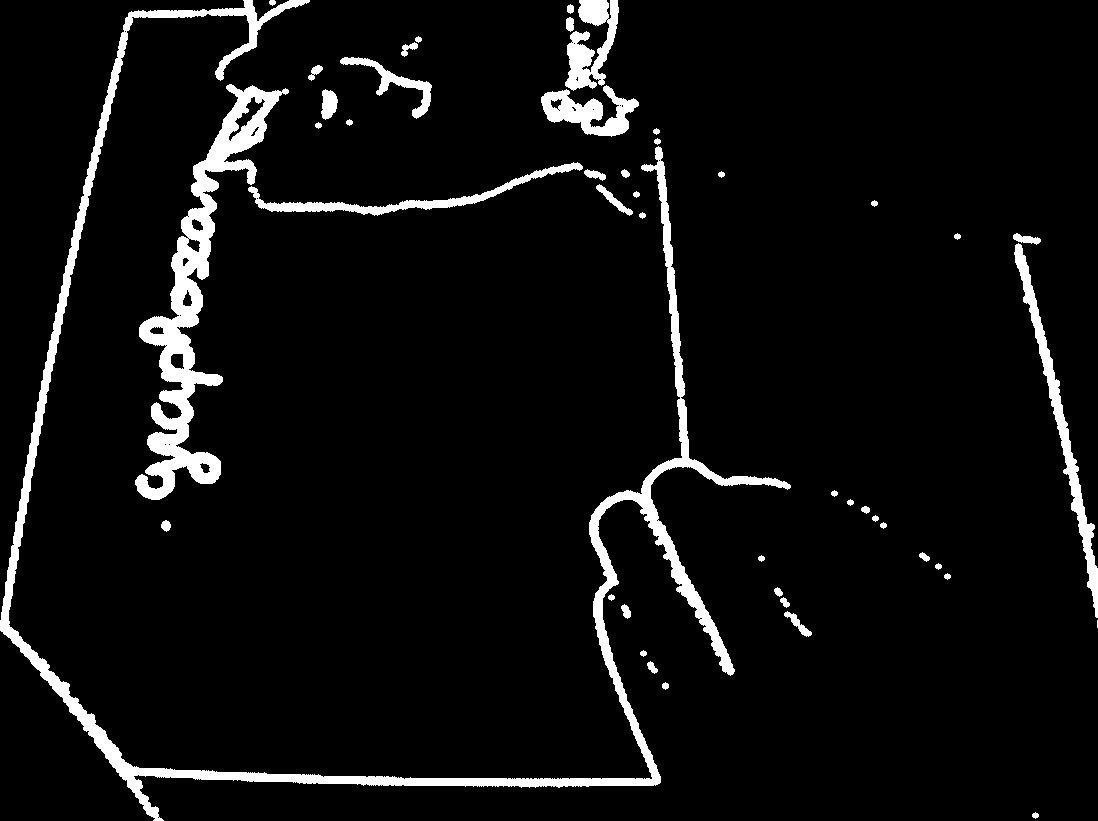
\includegraphics[width=\textwidth]{Modules/Picture/hog}
\caption{HOG brut}
\label{HOGSale}
\vspace{30px}
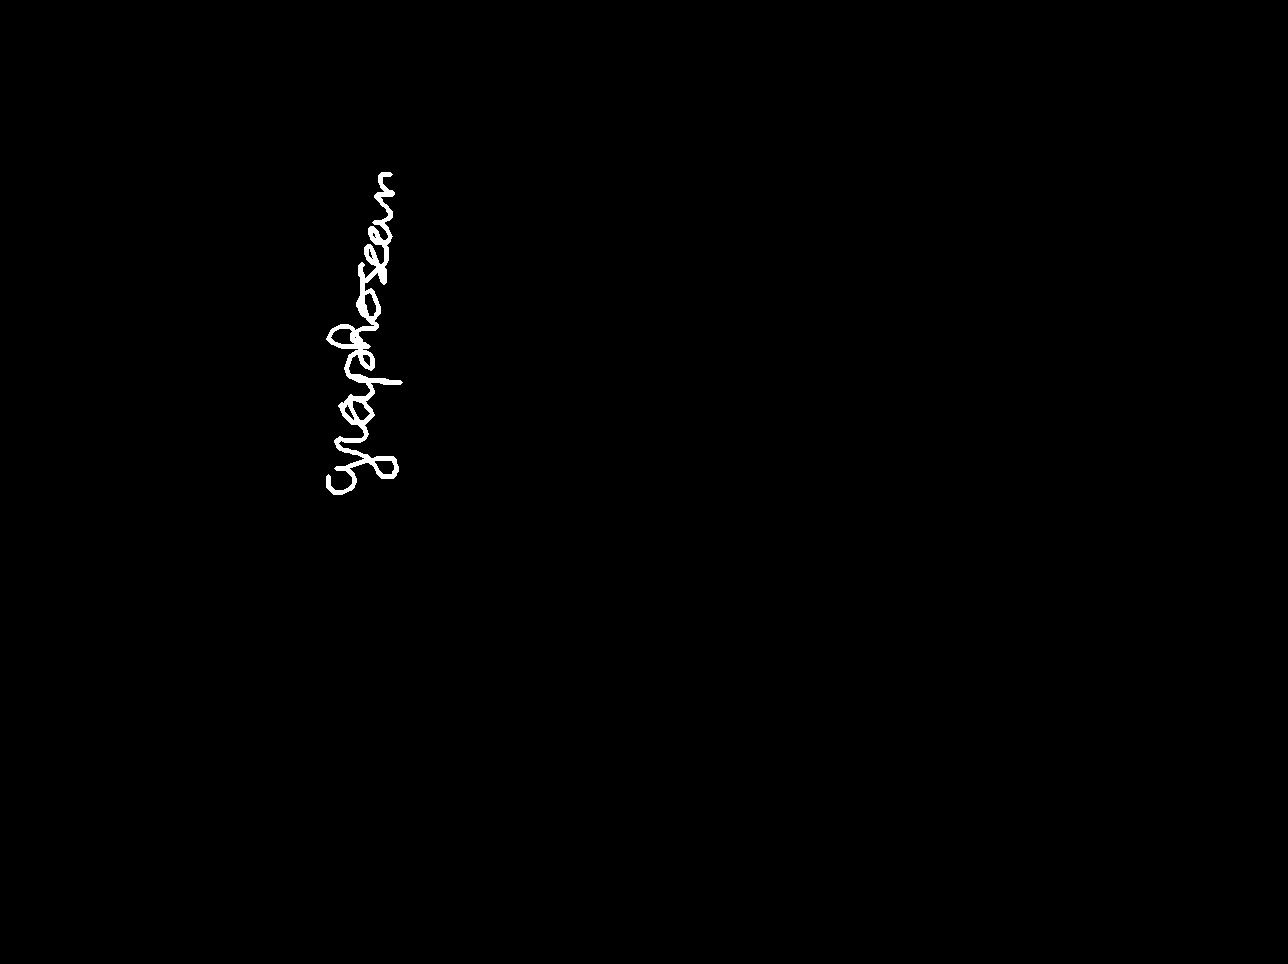
\includegraphics[width=\textwidth]{Modules/Picture/hog_propre}
\caption{HOG nettoyé}
\label{HOGPropre}
\end{figure}

\newpage

\begin{figure}
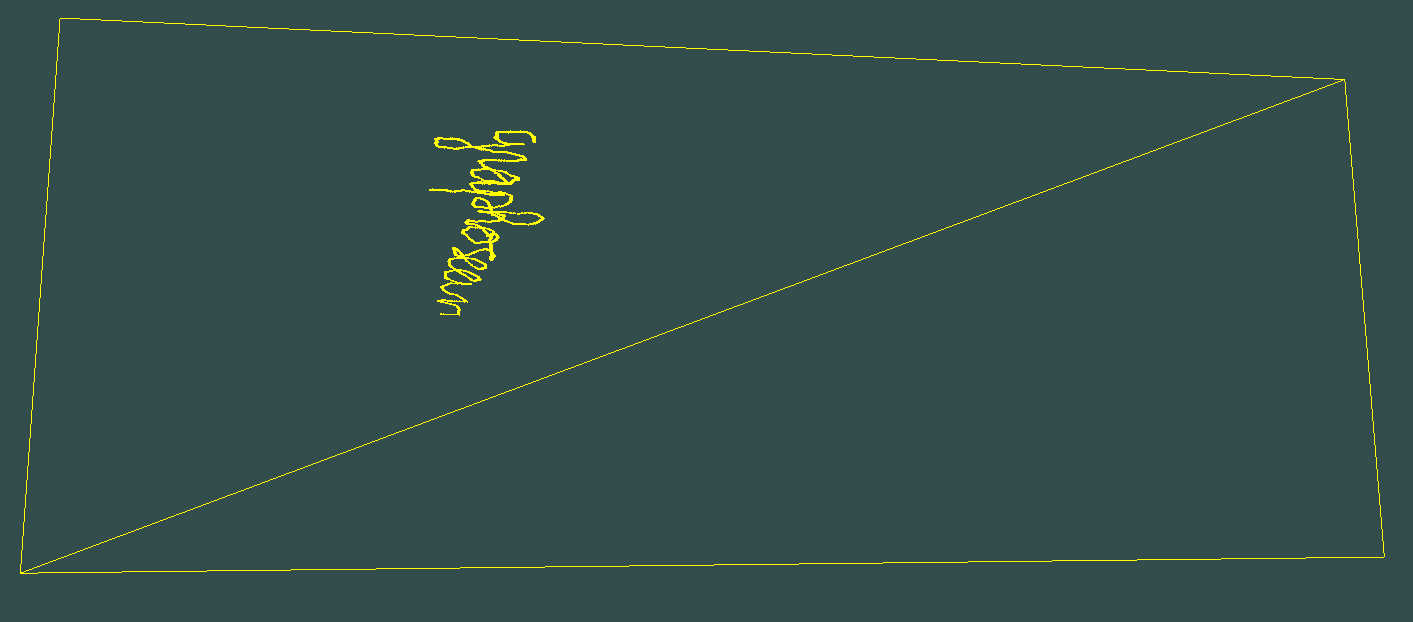
\includegraphics[width=\textwidth]{Modules/Picture/3d_1}
\caption{Image 3D - 1}
\label{3D1}
\vspace{30px}
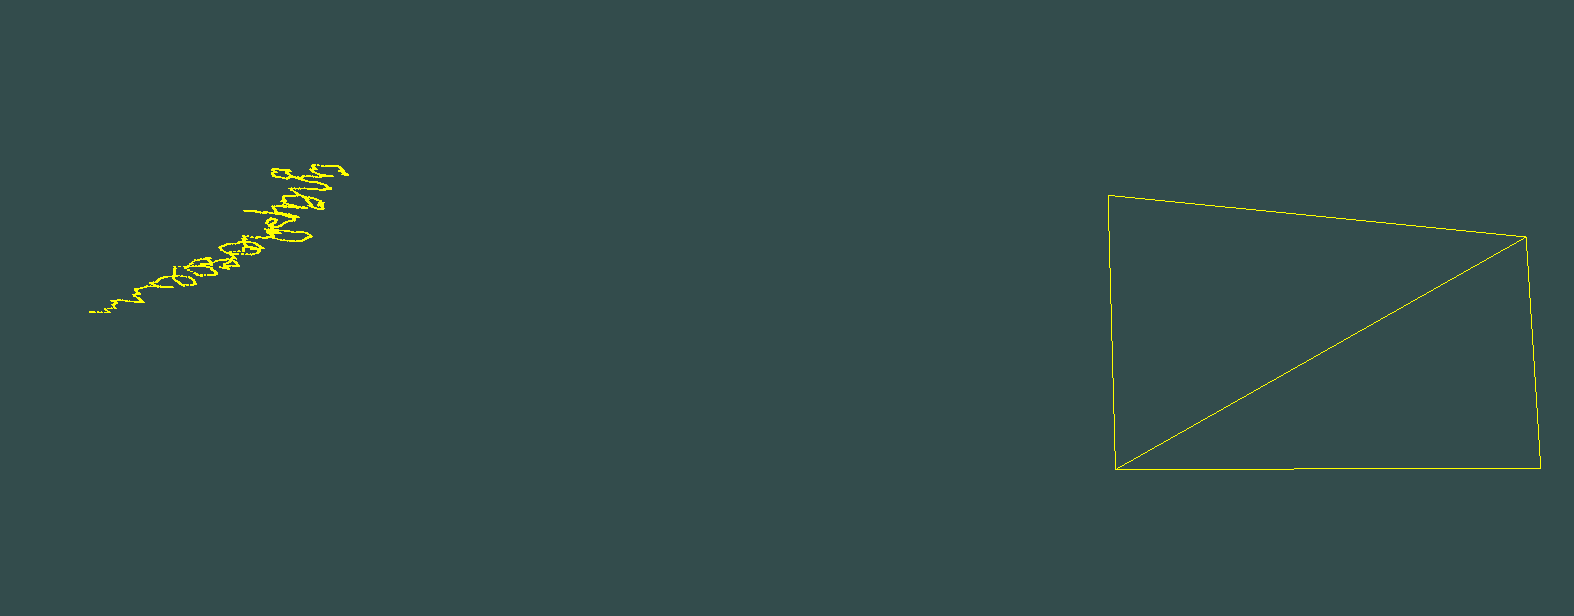
\includegraphics[width=\textwidth]{Modules/Picture/3d_2}
\caption{Image 3D - 2}
\label{3D2}
\end{figure}

\clearpage



\subsection{Langages et frameworks utilisés}

Le programme en lui-même est entièrement réalisé en C++, et différentes bibliothèques graphiques sont utilisées dans ce projet pour le traitement du flux vidéo, dans le but de faire du tracking sur le résultat, comme OpenGL et OpenCV. OpenGL est utilisé pour la reconstruction du mouvement de la plume en 3D, tandis qu'OpenCV est plus utilisé pour le traitement de l'image, notamment toutes les opérations faites dessus. De plus, Matlab est utilisé pour effectuer diverses opérations mathématiques sur les images, comme par exemple pour la calibration originelle servant à l'alignement pour la stéréo, ainsi que pour l'enlèvement de la distorsion. En effet, comme les caméras ont un grand angle, les éléments sur le bord de l'image sont courbés, il faut donc les remettre droits pour pouvoir travailler dessus.

\subsection{Fonctionnalités déjà implémentées}

Le programme tel qu'il nous a été fourni dispose de plusieurs fonctionnalités élémentaires permettant son bon fonctionnement. Parmi celles-ci, nous pouvons compter~:
\begin{itemize}
\item Le calibrage du dispositif dans sa globalité (caméras + surface d'écriture)
\item La synchronisation des deux caméras pour une reconstitution en trois dimensions des gestes lors de l'écriture
\end{itemize}
En plus de ces fonctionnalités, existe un dispositif matériel de capture. Ce dernier (Figure \ref{cameras}) est composé d'une structure en bois sur laquelle sont montées deux caméras. Ces dernières sont connectées à l'ordinateur par le biais d'un cable USB 3.0. Il est également possible de les bouger afin d'en ajuster les réglages.

\begin{figure}[!h]
\centering
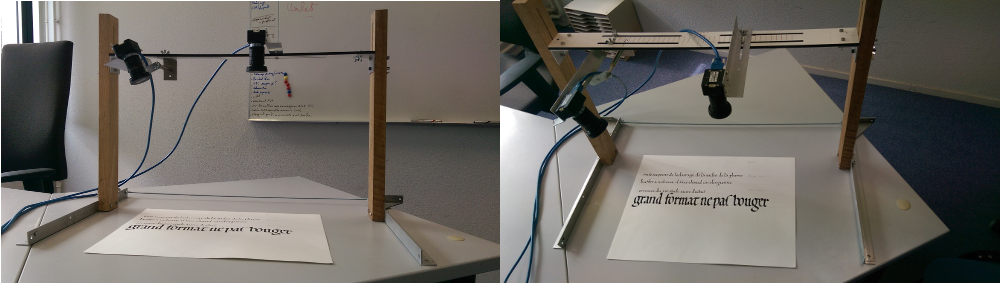
\includegraphics[width=\textwidth, height=4cm]{Modules/Picture/camerasPic.png}
\caption{Dispositif de capture stéréo}
\label{cameras}
\end{figure}

\subsection{Fréquence d'acquisition limitée}

Jusqu'alors, le programme ne possédait pas une fréquence d'acquisition suffisante de l'image. En effet, cette dernière n'était que de l'ordre de huit images par seconde. De ce fait, cette valeur ne permet pas une reconstituion précise en trois dimensions des gestes du calligraphe. L'objectif ici est donc de se rapprocher le plus possible de la fréquence maximale d'acquisition des caméras, soit trente images par seconde et ainsi gagner en précision lors du traitement.

\subsection{Impossibilité de bouger la feuille}

Avec la configuration actuelle, le calligraphe a l'impossibilité de bouger la feuille sur laquelle il écrit sous peine de perdre les réglages définis auparavant. Instinctivement, la personne qui écrit peut souhaiter bouger cette feuille et ainsi gagner en confort. Le but serait donc de trouver un moyen de gérer un changement de position de la feuille sans que cela n'affecte les résultats, en recalculant les réglages par exemple.

\subsection{Problèmes divers}

Initialement, l'éclairage du dispositif se faisait à l'aide de deux spots disposés de part et d'autre du calligraphe. Le problème majeur d'un tel moyen est la présence d'ombres à certains endroits rendant le traitement des images difficile, ainsi que la chaleur des lampes pouvant se réveler gênante à la longue. Un autre problème à gérer sont les gestes "inutiles" à l'acquisition que le calligraphe peut faire. En effet ce dernier peut par exemple vouloir étendre son bras pour se relaxer, geste qui sera pris en compte par le programme dans la reconstitution.

\section{Besoins fonctionnels et non fonctionnels}

	Une séparation des tâches était déjà effective dans le projet original, sur lequel travaillaient deux personnes : une personne s'occupait de l'acquisition stéréo, pendant que la seconde était sur la modélisation 3D de la plume. Cette séparation a été conservée dans ce TER : \textsc{Gallet} Benoît et \textsc{Herrmann} Emmanuel s'occupent de la première partie, tandis que \textsc{Charpignon} Thibault et \textsc{Réty} Martin ont pris la deuxième.

\subsection{Augmentation de la cadence d'acquisition}

Naturellement, différentes idées nous sont venues pour augmenter la cadence d'acquisition de la vidéo en stéréo. Nous les détaillons ici, même si par la suite cette liste sera sûrement étoffée. Le programme fonctionne suivant plusieurs étapes~: Tout d'abord, une image est capturée à partir des deux caméras, puis les deux images sont encodées dans une vidéo. Une fois la capture finie, la vidéo est traitée afin de régler les problèmes de distorsion. Grâce à cette grande boucle qui capture les images deux par deux (une image par caméra), les vidéos finales commencent et terminent exactement au même moment, et permettent donc d'avoir simultanément la feuille d'écriture filmée sous deux angles différents. La modélisation en 3D sous OpenGL est alors possible. La seule variable est que plus la cadence d'acquisition est élevée, plus il y aura de FPS sur les vidéos finales, et plus la modélisation 3D de la plume sera précise. De plus, notre architecture et notre code doivent être assez robuste, pour que si un jour une troisième voire une quatrième caméra soient rajoutées, le nombre de FPS ne redescende pas drastiquement.

\subsubsection{Programmation parallèle}

Grâce à la programmation parallèle, qu'elle soit au niveau du CPU avec de l'OpenMP ou des threads, ou au niveau du GPU avec CUDA, nous pensons pouvoir accélérer l'acquisition des images, et donc des FPS sur les vidéos finales. Nous pensons regarder quelles parties peuvent être faites en parallèle, peut-être est-il possible d'uniquement récupérer une image tous les 3 centièmes de secondes (pour les 30 fps) dans le programme principal, et de faire tous les autres traitements dans des régions parallèles, avec par exemple un thread qui s'occupe d'ajouter la prochaine image à la vidéo, un autre thread qui enlève la distorsion de l'image, etc.

\subsubsection{Complexité}

Reprendre le code pour en examiner sa complexité est une autre piste envisagée pour augmenter les FPS. Nous pensons séparer cette idée en deux étapes~: Tout d'abord regarder la complexité de l'algorithme dans sa généralité, pour se rendre compte s'il y a problème ou non à ce niveau là, et voir les morceaux posant plus problème que le reste, puis faire des tests plus précisément sur ces parties pour voir ce qui ne va pas. Une analyse légerement différente pourra être effectuée, avec des tests fontionnels calculant quelle partie prend le plus de temps. Ces tests sont très complémentaires de ceux de complexité, à eux deux ils devraient mettre en exergue les problèmes principaux du code actuel.

\subsubsection{Modularité}

Outre cette analyse de la complexité, une mise au propre du code devra être effectuée. En effet, tout se trouve dans la fonction \texttt{main}, dans deux grandes boucles. Une partie de notre travail sera donc de modulariser cette fonction, de la séparer en plusieurs méthodes afin de gagner en clarté. De plus, l'ajout de l'option \texttt{-O2} lors de la compilation permet d'optimiser sensiblement les performances. Nous prévoyons par la suite d'utiliser à la place \texttt{-O3} qui compilera les fonctions sur une seule ligne, ce qui permettra de minimiser le coût de cette modularisation du code lors de son exécution.

\subsubsection{Généralisation}

Sinon, le dernier axe sur lequel travailler sera la généralisation du nombre de caméras. Pour l'instant, tout dans le code est fait pour deux caméras, avec du code dupliqué pour chaque action. La généralisation pour \textit{n} caméras sera facilitée par la modularisation du code, et permettra par la suite de rajouter une ou plusieurs caméras sans modification majeure, uniquement en changeant quelques \texttt{\#define}.


\subsection{Tracking de la plume}

Comme pour la partie sur l'augmentation de la cadence d'acquisition, différents problèmes sont à résoudre pour le tracking. Cette partie permet de traiter les vidéos produites par les caméras et d'en ressortir une trace des mouvements effectués par le calligraphe. L'étudiant de Polytech qui a travaillé sur cette partie a recherché différents algorithmes permettant d'effectuer ce tracking. Son étude se focalise sur deux algorithmes basés sur l'apprentissage de toutes les apparences observées de l'objet et d'une estimation des erreurs pour ensuite les éviter:

\begin{itemize}

\item Tracking Learning Detection (TLD)

\item Kernelized Correlation Filters (KCF)

\end{itemize}

  
\subsubsection{Analyse de la complexité}

Heureusement, l'analyse des deux algorithmes a déjà été faite par l'étudiant, ce qui a montré que dans notre cas l'algorithme KCF est le plus efficace. Son étude est basée sur plusieurs critères, la déviation moyenne des deux vidéos, le nombre de frames et le temps de calcul. Seul le premier critère est réellement différent entre les deux méthodes. C'est cette différence qui a orienté son choix vers l'algortihme KCF. \\

Ici, notre premier axe de recherche sera orienté vers une étude complémentaire de ces algorithmes pour vérifier la véracité de l'analyse précédente. Pour cela nous allons réutiliser les critères d'études et ensuite essayer d'en trouver d'autres pour confirmer le choix. Dans un second temps il nous faudra rechercher d'autres algorithmes ou méthodes de programmation pour améliorer le tracking.

\subsubsection{Gestion mouvements}

Bien entendu, le choix des algorithmes n'est pas la seule difficulté, nous faisons face également à des contraintes physiques liées aux mouvements du calligraphe. Par exemple il doit prendre des temps de repos afin de garder sa fluidité d'écriture en faisant des gestes de relaxation du poignet. Ces mouvements ne doivent pas être pris en compte par l'algorithme de tracking afin d'éviter des erreurs sur la représentation du mouvement. \\

Résoudre ce problème ce problème pourrait passer par la sauvegarde à un temps T et à un temps T+1 d'une image de la partie suivie. Puis analyser la différence entre les deux images et en ressortir un résultat positif ou négatif. Cela reviens à prendre la dernière image où le calligraphe écrit et une autre image qui permettra de voir si le mouvement est la continuité de l'écriture ou un mouvement parasite.

\subsection{Autres axes de travail}

\subsubsection{Zone de capture}

En écrivant, le calligraphe doit de temps en temps bouger la feuille pour se repositionner et continuer sa rédaction. L'algorithme actuel ne gère pas ce mouvement, ce qui nécessitait après chaque mouvement de la feuille un nouveau calibrage des caméras et de la zone de capture. Une solution possible pour résoudre ce problème est la mise en place d'un système de cadre pour que le calligraphe sache la zone dans laquelle il peut écrire. Ce cadre pourrait être un marquage sur la feuille qui délimitera la zone de capture. Nous souhaitons également rechercher d'autre solutions possibles pour résoudre ce problème.

\subsubsection{Changement de la structure}

Pour le moment le dispositif de capture ne comporte que deux caméras et des angles de prises de vue bien définis. L'ajout d'une caméra et le repositionnement des deux premières peut permettre de rendre plus précise l'acquisition. De cette manière nous aurions à notre disposition des informations supplémentaires pour améliorer la reconstruction du mouvement. Il nous faut donc tester différentes configurations et choisir la meilleure \\

Un des facteurs majeurs de la capture d'image est la lumière. En effet, il est important que la feuille soit bien éclairée pour le confort et l'écriture du calligraphe. La structure actuelle ne comporte pas d'éclairage du tout, il était nécessaire d'avoir une lampe d’appoint. Une solution simple est l'ajout d'une plaque LED pour avoir une luminosité uniforme sur toute la feuille. \\

Tous ces changements devront peut-être être accompagnés d'une refonte totale du dispositif.

\subsubsection{Compatibilité Windows - Linux - MacOS}

A l'origine, les étudiants ont développé tout le code sur Windows et plus particulièrement sur l'IDE Visual Studio (C++). Pour rendre le code réutilisable à l'avenir nous avons comme objectif de pouvoir l'utiliser sur tous les systèmes d'exploitation (Linux/MacOS en plus). Pour cela il est nécessaire d'uniformiser le code et de se servir de librairies communes pour standardiser au mieux le projet.

\section{Prototypes et résultats de tests préparatoires}

Il nous fallait, pour bien prendre en main le projet, tester réellement le dispositif de lancement du logiciel jusqu'à la capture vidéo. Nous avons dû  procéder à l'installation de tout l'environnement de travail nécessaire (FlyCap2, OpenCV, OpenGL) et l’acquisition des premières vidéos avec les caméras mises à notre disposition. \\

Notre première tâche a été de transférer le code initial sous Linux et ainsi le tester directement. Les tests ont été concluants et le premier groupe a pu commencer directement à améliorer le système. Le second, quant à lui, a récupéré le code concernant le tracking mais a rencontré de gros problèmes lors de son passage de Windows vers Linux.
Le code n'utilisant pas des fonctions standards, important des librairies en "dur" et étant peu commenté, il est pour le moment impossible de tester le code de l'étudiant qui travaillait sur le tracking l'année précédente. Pour y remédier le second groupe a dû repasser cette partie du projet sur Windows le temps de bien comprendre les différents problèmes et de les corriger.

\section{Architecture}

Le projet est scindé en deux grosse parties, presque indépendantes l'un de l'autre.
Comme montré dans la figure \ref{architecture} , toute l'acquisition des vidéos se fait en parallèle dans la partie acquisition. Cette partie gère aussi l'undistortion des vidéos. Une fois les vidéos créées et traitées correctement, on peut les envoyer à la seconde grosse partie qui est celle du tracking/reconstruction 3D. Cette partie permet de gérer différentes choses, comme des types de tracking ou de la reconstruction en OpenGL. Cette classe fonctionne comme une boîte noire, que l'on peut paramétrer à loisir pour réaliser ce dont on a besoin.

\subsection{Acquisition}
L'acquisition est elle-même séparée en deux parties. La première est l'ac\-qui\-si\-tion à proprement parler, elle récupère le flux vidéo des deux caméras et permet de les synchroniser. Les vidéos sont encodées en avi, image par image, au rythme de 30 fps, ce qui est la cadence maximum des caméras.

Une fois les vidéos synchrones créées, de l'undistortion est appliquée dessus. En effet, comme les caméras possèdent un grand angle, les bords sont déformés, il faut donc les remettre droits.

\subsection{Tracking et reconstruction}

Les vidéos créées sont ensuite passées au deuxième programme. Celui-ci peut exécuter différentes fonctions sur les vidéos. Une classe HOG permet de faire de la reconnaissance d'image, et une classe GraphoScan permet de lancer les différents trackings. Pour l'OpenGL, la classe Shader permet de compiler des shaders tandis qu'OpenGL permet de dessiner les points dans le repère. Enfin, Camera sert à exécuter les différents mouvements de la caméra (zoom, direction, ...).

\begin{figure}[!htb]
\centering
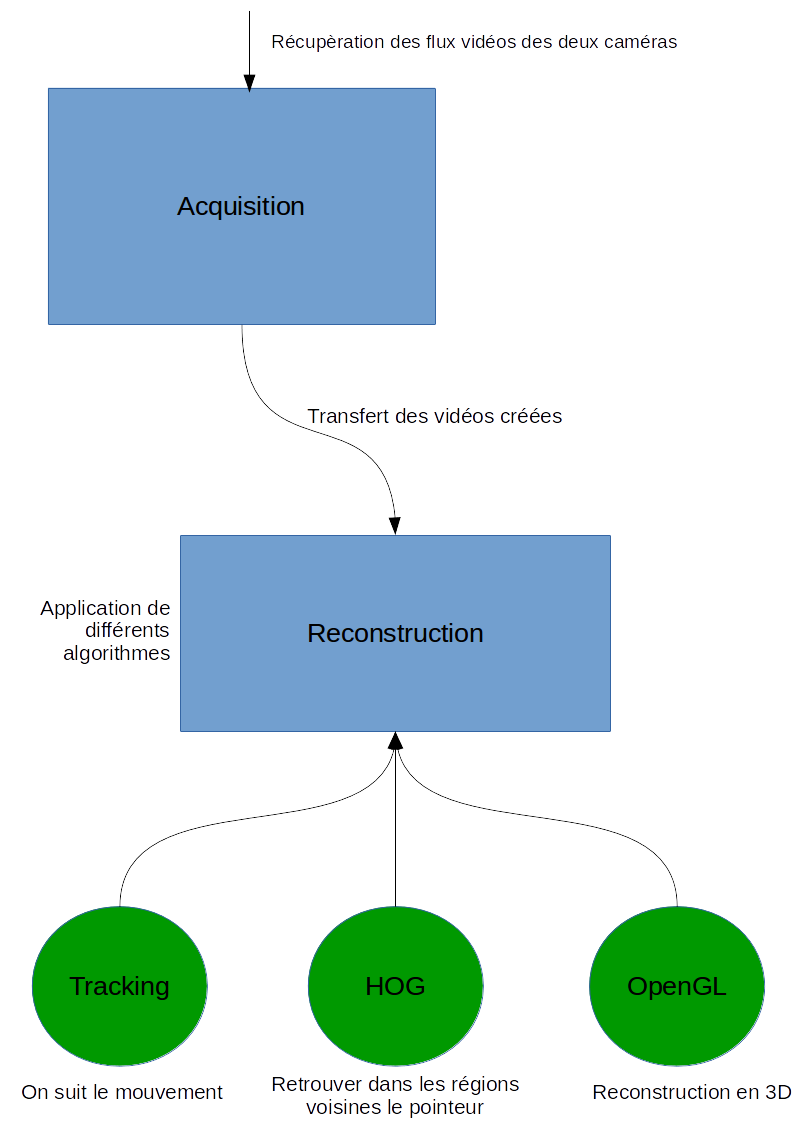
\includegraphics[width=\textwidth]{Modules/Picture/Architecture.png}
\caption{architecture}
\label{architecture}
\end{figure}

\clearpage

\section{Algorithmes et structures de données}

\subsection{Parallélisation OpenMP}
Afin de pouvoir faire de l'acquisition vidéo en simultané sur plusieurs caméras tout en gardant le plus possible d'images par seconde, nous avons opté pour une parallélisation de l'algorithme d'acquisition grâce à OpenMP. Ainsi nous affectons - dans la mesure du possible - une caméra à un thread en lançant la région parallèle de cette sorte :
\begin{verbatim}
#pragma omp parallel num_threads(numCameras)
\end{verbatim}
Avec \texttt{numCameras} le nombre de caméras détectées. \\
Juste avant de commencer la capture, nous posons une barrière à l'aide de 
\begin{verbatim}
#pragma omp barrier
\end{verbatim}
dans le but de déclencher la capture des caméras de la manière la plus synchronisée possible.
À l'intérieur de la boucle d'acquisition, une nouvelle barrière est mise avant chaque récupération du buffer de la caméra.
Dans le cas où l'utilisateur souhaite faire un affichage de la capture qu'il est en train d'effectuer, un des threads est choisi via
\begin{verbatim}
#pragma omp single
\end{verbatim}
afin de s'occuper de cet affichage.
Enfin, chaque thread écrit la frame dans la vidéo correspondant à sa caméra.

\subsection{Export des paramètres de la caméra}

La récupération des paramètres de la caméra, calculés via MatLab, va nous permettre de faire l'undistortion et la reconstruction 3D. Jusqu'à présent, ces paramètres étaient rentrés en dur dans les programmes, nous avons donc décidé de faire des imports/exports de ces données pour plus de simplicité et de ré\-u\-ti\-li\-sa\-bi\-li\-té.
Pour ce faire, une fois les paramètres de calibration calculés dans MatLab , on récupère un objet CameraParameters par caméra. Afin de générer les fichiers de configuration nécessaires, il suffit de rentrer deux commandes par caméra :

\begin{verbatim}
	dlmwrite( 													  \
	'*PATH_TO_ACQUISITION*/Calib_camera_*NUM_CAMERA*_Matlab.txt', \
	camera*NUM_CAMERA*.IntrinsicMatrix,'delimiter', ' ',		  \
	'precision', 5)
	dlmwrite(													  \
	'*PATH_TO_ACQUISITION*/Calib_camera_*NUM_CAMERA*_Matlab.txt', \
	horzcat(camera*NUM_CAMERA*.RadialDistorsion,				  \
	camera*NUM_CAMERA*.TangentialDistorsion),					  \
	'-append', 'delimiter', ' ', 'precision',5)
\end{verbatim}

Il faut remplacer $*NUM\_CAMERA*$ par le nom de l'objet de la caméra correspondante.

\subsection{Tracking}

De nombreux algorithmes de tracking existent, dans ce projet nous en utilisons plusieurs, tous fournis par OpenCV:
\begin{itemize}
\item KCF (High-Speed Tracking with Kernilized Correlation Filters) utilise les propriétés des matrices circulantes pour faire son tracking. (cf \cite{kernelized_correlation_filters})
\item TLD (Tracking Learning Detection) suit l'objet voulu image par image et grâce à une comparaison avec toutes les apparences observées réajuste le tracker de la cible. 
\item MIL (Multiple instance learning) crée et enrichie un classifieur pour sé\-pa\-rer l'objet suivi et le reste de l'image.
\item Boosting, comme MIL, utilise des classifieurs pour savoir où est l'objet et où sont les éléments extérieurs. 
\end{itemize}
Il y a également d'autres algorithmes mais nous n'avons pas eu le temps de les tester.
L'étudiant précédent a fait une comparaison entre l'algorithme KCF et TLD, à l'aide du comparatif des méthodes de tracking existantes, proposé par Joao F.Henriques et de quelques tests, il en est ressorti que KCF était plus efficace que TLD. 
Toutefois nous nous sommes également penché sur ce sujet. Pour savoir si un algorithme de tracking est plus efficace qu'un autre nous les avons comparés sur différents critères: 
\begin{itemize}
\item La perte ou non du tracker sur la cible.
\item La taille du tracker nécessaire pour avoir un tracking.
\item Le suivi de certains mouvements.
\item La rapidité d'exécution de l'algorithme.
\end{itemize}
Après avoir défini ces critères nous avons commencé les tests sur les mêmes vidéos à 30 fps. Ces tests ont donné des résultats complètement différents pour chaque algorithme. Il faut toutefois relativiser ces tests à la taille de la ROI. En effet, plus celle-ci est grande, et plus l'algorithme sera lent à l'exécution.

KCF est l'algorithme le plus stable, le tracker suit parfaitement la cible tant que celle-ci n'effectue pas un mouvement trop rapide. C'est également celui qui a le temps d'exécution le plus rapide. Après analyse de son code (OpenSource), nous avons ressorti une complexité d'environ $O(n^{4})$, toutefois cette analyse fut rapide et nous n'avons pas eu le temps de l'approfondir.
Boosting et MIL, qui utilisent la même technique d'apprentissage et d'enrichissement de classifieurs, donnent les mêmes résultats. Le choix de la région d'interêt (ROI) a un impact significatif sur le tracking. L'utilisation d'un multi-tracker favorise l'analyse de l'image et ressort un tracking efficace, de plus la sélection d'une grande ROI n'a pas de réel impact.
TLD donne des résultats complètement différents selon la situation. Lors d'un tracking sur des mouvements simples, celui-ci est le moins efficace de tous. En effet, il recalcule la ROI à chaque frame ce qui est très coûteux et modifie le résultat final du tracking. Toutefois lors de mouvements rapides, qui ne sont pas gérés par les autres algorithmes, TLD arrive à retrouver  l'objet grâce à sa base de connaissance.

A partir de tous ces tests nous en avons conclu que le choix de l'algorithme dépend de l'objet que l'on veut suivre. Si celui-ci est simple à observer, KCF est le plus approprié, mais lorsqu'il commence à être plus compliqué à suivre, il est préférable de se tourner vers les autres algorithmes qui utilisent leurs bases de connaissances pour retrouver l'objet.

\subsection{Fonctionnement de la reconstruction 3D}

Pour faire la reconstruction nous avons gardé les différentes librairies utilisées dans le code fourni. Nous avons utilisé GLFW 3 comme libraire de gestion de fenêtre et de contexte OpenGL, GLM comme librairie mathématique permettant de manipuler des matrices de toute taille et GLEW comme librairie de gestion des extensions utilisées et surtout pour gérer la plateforme sur laquelle on utilise OpenGL. \\
 
La reconstruction 3D de ce qui est écrit dans la vidéo capturée se fait en fin de programme. Le tracking produit un fichier de points 3D qui sont utlisés pour la reconstruction avec OpenGL. Ce programme s'effectue en deux phases. \\

\subsubsection{Initialisation de la fenêtre et du contexte OpenGL}
La première phase consiste à initialiser les outils OpenGL utilisés. Dans un premier temps il a fallu initialiser la fenêtre OpenGL, c'est à dire attribuer la version d'OpenGL utilisée, une taille, et même lier les fonctions d'évenement OpenGL (mouvement de souris, touches clavier, etc) à la fenêtre. Ensuite il y a une initialisation du contexte, c'est à dire créer les outils qui permettent de lier les points 3D, la fenêtre et d'autres valeurs à la carte graphique (GPU). Pour cela on utilise des Vertex Array Object (VAO) qui permettent de lier à la carte graphique un programme nommé Shader, composé de FragmentShader qui sont utilisés pour dessiner dans la fenêtre. On utilise également des Vertex Buffer Object (VBO) qui nous permettent de lier des variables (ou structures) stockées dans le processeur (CPU) avec la GPU, qui permettront d'influer sur ce qui est dessiné dans la fenêtre par le Shader. \\

\subsubsection{Dessin des points dans le repère 3D}
La deuxième phase est la phase de traitement des données. Dans un premier temps il a fallu \textit{parser} le fichier dans lequel les points 3D sont contenus. Ensuite nous avons chargé dans deux VAO différents deux Shaders, un qui sera utilisé pour construire un plan dans le repère 3D et un second qui sera utilisé pour effectuer le dessin des points 3D du tracking. Pour le dessin des points lors du \textit{parsing} nous plaçons chaque point dans des matrices à quatre lignes et une colonne qui contiendront les coordonnées du repère x,y,z et w. Une fois la liste remplie nous plaçons le point dans la fenêtre OpenGL à l'aide d'un savant calcul de placement de point qu'on nommera PVM. Ce PVM n'est rien d'autre qu'une suite de multiplications de matrices ordonnées : matrice de projection * matrice de vue * matrice de modèle qui permettent de rendre visible un dessin dans une fenêtre en fonction de la position de la camera et des coordonnées du point à dessiner.
La matrice du modèle (M) est obtenue par la translation T , la rotation R appliquée sur l'objet tel que : $R * T * v = M * v$ où v est un vecteur de l'objet.
La matrice de vue (V) est obtenue par la multiplication de M et un alignement des objets de la fenêtre par rapport à la vue humaine : $v' = V * M * v$ où v est un vecteur de l'objet.
La matrice de projection (P) est obtenue par la multiplication de V, M, et une projection dans la fenêtre des objets : $v' = P * V * M * v$ où v est un vecteur de l'objet.
Une fois ces valeurs de PVM envoyées à la GPU, le point est alors dessiné et est visible sur la fenêtre.
Pour le dessin du plan nous avons repris les paramètres PVM calculés precedement, puis effectué le dessin des points placés dans le repère.
Nous avons alors en visuel le plan et ce qui a été reconstruit en 3D, une représentation de l'écriture effectuée dans la vidéo. Il est alors possible de bouger dans la fenêtre avec des touches et d'orienter sa vue en fonction de la position de la souris.

\section{Complexité}

\subsection{Acquisition}

\subsubsection{Acquisition stéréo et enregistrement des vidéos}

On assume le fait qu'il y ait n lignes et m colonnes dans une image. Nous proposons deux complexités, une borne min si on considère qu'un pixel de l'image se traite en temps $O(1)$, et une borne max si l'on considère que le pixel se traite en temps $O(3)$ à cause de ses caractéristiques RGB.

\textbf{Borne min}

Récupération de l'image brute (RetrieveBuffer) : $O(n*m)$

Conversion de l'image brute vers RGB (rawImage.Convert) : $O(n*m)$

Création de la matrice de l'image RGB (imageRGB=cv::Mat) : $O(n*m)$

Ecriture d'une image dans la vidéo (outputVideo.write) : $O(n*m)$

Ce qui nous donne un total de temps d'exécution en $O(4(n*m))$.

\textbf{Borne max}

Il suffit de multiplier par trois les valeurs précédentes, ce qui nous donne au total $O(12(n*m))$

\textbf{Analyse}

Nous pouvons donc en conclure que le temps d'exécution de l'algorithme C est :
$O(4(n*m)) \leq C \leq O(12(n*m))$

C'est-à-dire qu'il s'exécute globalement en temps linéaire en la taille de l'entrée. Cela dit, il faut l'exécuter à chaque tour de boucle (à chaque acquisition d'image), donc on pourrait dire que sa complexité serait alors de $O(n*m*f)$, f étant le nombre de frames que nous enregistrons. Evidemment, cela vaut pour la version parallèle du code, si on prend en compte la version séquentielle, il faut bien sûr multiplier cette complexité par le nombre de caméras que l'on a.

\subsubsection{Tracking}

De nombreux algorithmes de tracking existent, dans ce projet nous utilisons différents algorithmes fournis par OpenCV:
\begin{itemize}
\item KCF (High-Speed Tracking with Kernilized Correlation Filters) utilise les propriétés des matrices circulantes pour faire son tracking. (cf papier sur KCF)
\item TLD (Tracking Learning Detection) suit l'objet voulu image par image et grâce à une comparaison avec toutes les apparences observées réajuste le tracker de la cible. 
\item MIL (Multiple instance learning) crée et enrichie un classifieur pour séparer l'objet suivi et le reste de l'image.
\item Boosting, comme MIL, utilise des classifieurs pour savoir ou est l'objet et ou est les éléments extérieurs. 
\end{itemize}
Il y a également d'autres algorithmes mais nous n'avons pas eu le temps de les tester.
L'étudiant précédent a fait une comparaison entre l'algorithme KCF et TLD, à l'aide  du comparatif des méthodes de tracking existants proposé par Joao F.Henriques et de quelques tests, il en a ressorti que KCF  était plus efficace que TLD. 
Toutefois nous nous sommes également penché sur ce sujet. Pour savoir si un algorithme de tracking est plus efficace qu'un autre nous avons les avons comparé sur différents critères: 
\begin{itemize}
\item La perte ou non du tracker sur la cible.
\item La taille du tracker nécessaire pour avoir un tracking.
\item Le suivi de certain mouvement
\item La rapidité d'exécution de l'algorithme
\end{itemize}
Après avoir défini ces critères nous avons commencer les tests sur les même vidéos à 30 fps. Ces tests ont donné des résultats complètement différent pour chaque algorithme.
KCF est l'algorithme le plus stable, le tracker suit parfaitement la cible tant que celle-ci n'effectue pas un mouvement trop rapide. Il est également celui-ci qui le temps d'exécution le plus rapide. Après analyse du code OpenSource  permettant de l'exécuter, nous avons ressorti une complexité d'environ $O(n^{4})$, toutefois cette analyse fut rapide et nous n'avons pas eu le temps de l'approfondir.
Boosting et MIL, qui utilisent la même technique d'apprentissage et d'enrichissement de classifieurs, donnent les même résultats. Le choix de la région d'interêt (ROI) a un impact significatif sur le tracking. L'utilisation d'un mutli-tracker favorisait leur analyse de l'image et ressortait un tracking efficace et la sélection d'une grande  ROI n'avait pas de réel impact.
TLD donne des résultats copmlètement différent celon la situation. Lors d'un tracking sur des mouvements simple celui-ci est le moins efficace de tous, il recalcule la ROI à chaque frame ce qui est très coûteux et modifie le résultat final du tracking. Toutefois lors de mouvements rapides, qui ne sont pas gérés par les autres algorithmes, TLD arrive à retrouver  l'objet grâce à sa base de connaissance.
A partir de tous ces tests nous en avons conclu que le choix de l'algorithme dépend l'objet que l'on veut suivre. Si celui-ci est simple à observer KCF est le plus approprié, mais lorsque celui-ci commence à être plus compliqué à suivre il vaut mieux se tourner vers les autres algorithmes qui utilisent leurs bases de connaissances pour retrouver l'objet.


\section{Tests de fonctionnement et de validation}

Différents tests de validation ont été effectués tout au long du projet afin de s'assurer du bon fonctionnement de l'application. Ces tests pourront être refaits par la suite en décommentant les $\sharp$ define nécessaires, et pourront donc être réutilisés par des étudiants reprenant ce projet.

\subsection{Latence}

La latence est une caractéristique incontournable de notre projet, le client nous ayant précisé plusieurs fois que c'était très important qu'il y ait le moins de décalage possible entre les deux vidéos. Plus le décalage est grand et moins la reconstruction en 3D par la suite sera précise. Nous avons donc mesuré précisément le temps qui sépare deux frames dans le code. 

\begin{figure}[!h]
\centering
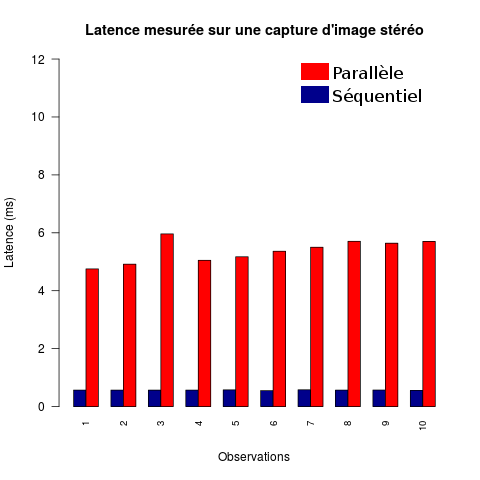
\includegraphics[width=\textwidth, height=10cm]{Modules/Picture/latence.png}
\caption{Latence}
\label{latence}
\end{figure}

Ce diagramme en bâton (Figure \ref{latence}) montre cette latence. Elle est plus importante avec le parallélisme qu'avec le programme séquentiel. Il faudra donc que le client pèse le pour et le contre sur la méthode qu'il préfère utiliser. Avec le parallelisme, le nombre de caméra pourra être augmenté (de façon raisonnable) sans chute de fps, car chaque coeur de la machine s'occupera d'une caméra particulière, par contre, la latence est plus importante(5 à 6 ms) . Avec la version séquentielle du code, la latence est plus que minime (1/2 millième de seconde environ), mais l'ajout d'une à plusieurs caméras fera chuter le nombre de fps.
De plus, la latence sera surement plus constante dans la région parallèle, car chaque thread s'occupant d'une caméra, celle-ci n'augmentera pas si on ajoute plus de caméras (dans la limite des coeurs disponibles sur la machine). Par contre, séquentiellement, comme on lance les acquisitions les unes après les autres, plus il y a de caméras, plus celles qui sont lancées en dernier auront de décalage avec la première.

\subsection{FPS}

\section{Extensions et améliorations possibles}

\subsection{Droits d'auteur}
Au fur et à mesure que nous essayions de comprendre le code de la reconstruction 3D (ce qui a été long car il a été fourni sans doc, commentaires et explications d'utilisation, avec une syntaxe et des imports pour Windows), nous nous sommes rendu compte que sur cette partie plusieurs morceaux de code avaient été copiés sur Internet.

La classe Shader, ainsi que la moitié de la classe Camera provient de \url{http://blog.csdn.net/sinat_26989191/article/details/51205149}, un outil pour faire un système solaire en 3D.

La classe HOG est presque entièrement copié collée de la fin de ce programme ( \url{http://lib.csdn.net/snippet/cplusplus/28974} ), qui est sous copyright.

Diverses autres parties du code proviennent de copiés-collés de différentes documentations ou exemples, ce qui est dans une certaine mesure moins dé\-ran\-geant.

Il y a certainement d'autres endroits du projet qui proviennent d'Internet, tout n'a pas été vérifié par manque de temps. Au total, nous estimons qu'au moins 50\% du code n'a pas été écrit par le groupe précédent. Cela implique que si ce projet est repris par un groupe futur, il faudra réécrire ces parties du code, ou du moins indiquer clairement les sources et les différents copyrights sur les classes copiées.

\subsection{Interface graphique}

Une extension possible serait de réaliser une interface graphique, par exemple en Qt. Cela permettrait un maniement beaucoup plus facile de l'application, et rendrait possible son utilisation par des personnes extérieures. En effet, en ce moment tout s'exécute dans le terminal, ce qui peut être moins intuitif. Avec cette interface graphique, on pourrait par exemple choisir de sélectionner une caméra pour voir ce qu'elle enregistre, définir différentes options comme choisir l'algorithme de tracking à utiliser, les sorties vidéos ou images à effectuer, ...

\subsection{Améliorer le code}

Nous avons 

\section{Bilan}

Nous avions différents objectifs au départ, concernant les deux parties de notre TER, acquisition et tracking/reconstruction.

Le premier était d'avoir une vidéo à 30 fps. Précedemment, le programme capturait les images à la vitesse de 7 ou 8 images/secondes, et actuellement on crée des vidéos en 30 fps constants, et en plus avec de la parallélisation, ce qui nous laisse à penser que le nombre de caméras peut augmenter sans baisser ce chiffre.

Il fallait ensuite généraliser le code de l'acquisition pour qu'il puisse marcher pour n caméras. Au départ, tout était fait pour deux caméras, avec du code copié-collé en deux fois pour chacune des caméras. Tout cela a été modifié, avec des tableaux de taille n (pour n caméras). Par contre, pour la partie reconstruction 3D, cela marche toujours avec deux caméras. Pour modifier cela, il faudrait changer la méthode de reconstruction 3D de points qui actuellement ne prend les points que de deux caméras. Une autre solution serait de lancer le programme sur toutes les paires de caméras et de faire ensuite la moyenne des points récoltés pour plus de réalisme dans la reconstruction.

Le code devait être compilable et exécutable sous environnement UNIX, les étudiants précédents l'ayant fait marcher uniquement sous Windows. Ce point a été également réalisé, une partie de ce rapport (section Manuel) a même été fait pour permettre aux prochains étudiants qui travailleront sur ce projet d'installer les frameworks et bibliothèques nécessaires à la compilation du code, ainsi que des explications sur l'utilisation de l'application.

Pouvoir bouger la feuille n'a malheureusement pas pu être fait par manque de temps, cependant nous avons réfléchi à une solution pour le faire, qui est détaillée dans la partie Extensions et améliorations possibles.

Il fallait rendre le code plus lisible. Ceci a également été fait, grâce à un gros travail de documentation et de compréhension du code. En effet, la majeure partie n'était pas commentée, avec des noms de variables non explicites, etc. Cela a été amélioré, avec une documentation Doxygen, afin que le code puisse être compris par tous.

Enfin, en naviguant sur la documentation de PointGrey (le fabricant des caméras), nous nous sommes rendu compte qu'il existait déjà un moyen de faire de l'acquisition stéréo, grâce à des fonctions dans l'API fournie, et à un cable reliant les caméras. Peut-être faudrait-il envisager aussi cette solution dans le futur, même si notre travail d'amélioration du code de l'étudiant précédent s'étant occupé de cette partie est désormais finie.



\section{Planning}

Les petites barres sur les diagrammes de Gantt (Figure \ref{gantt} et suivantes) correspondent aux différentes réunions que l'on a eu, suivies des noms des participants. Les plus grandes correspondent quant à elles aux tâches effectuées. Il y en a peu pour le moment car la phase de compréhension et d'installation des composants a été relativement longue.

\newpage
\begin{figure}
	\begin{center}
		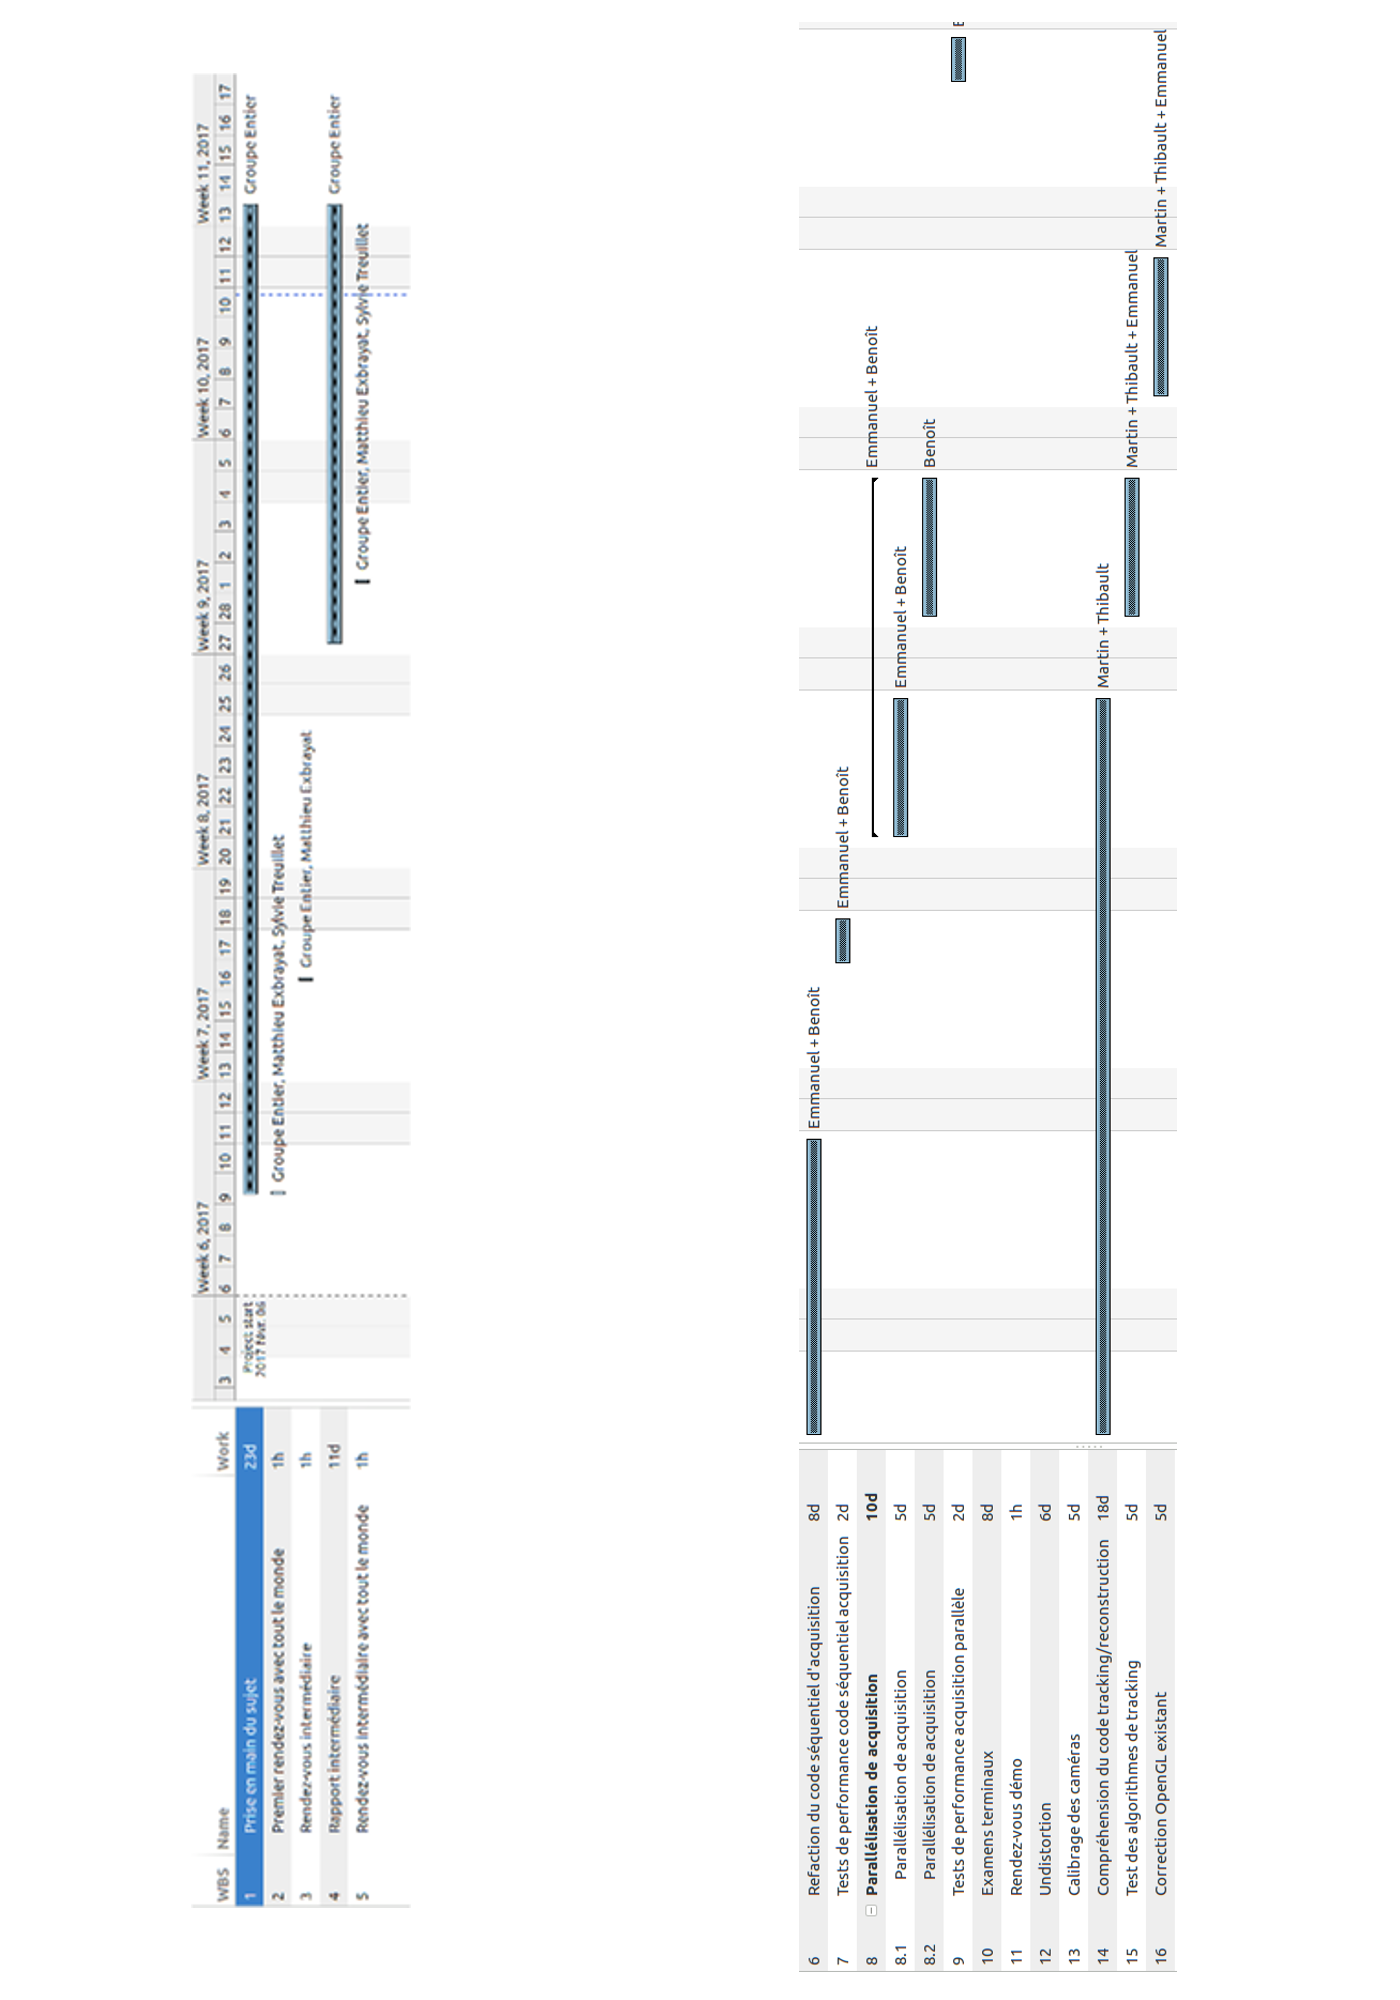
\includegraphics[scale=0.3]{Modules/Picture/gantt_0_1}
		\caption{Diagramme de Gantt 1/2}
		\label{gantt}
	\end{center}
\end{figure}

\newpage
\begin{figure}
	\begin{center}
		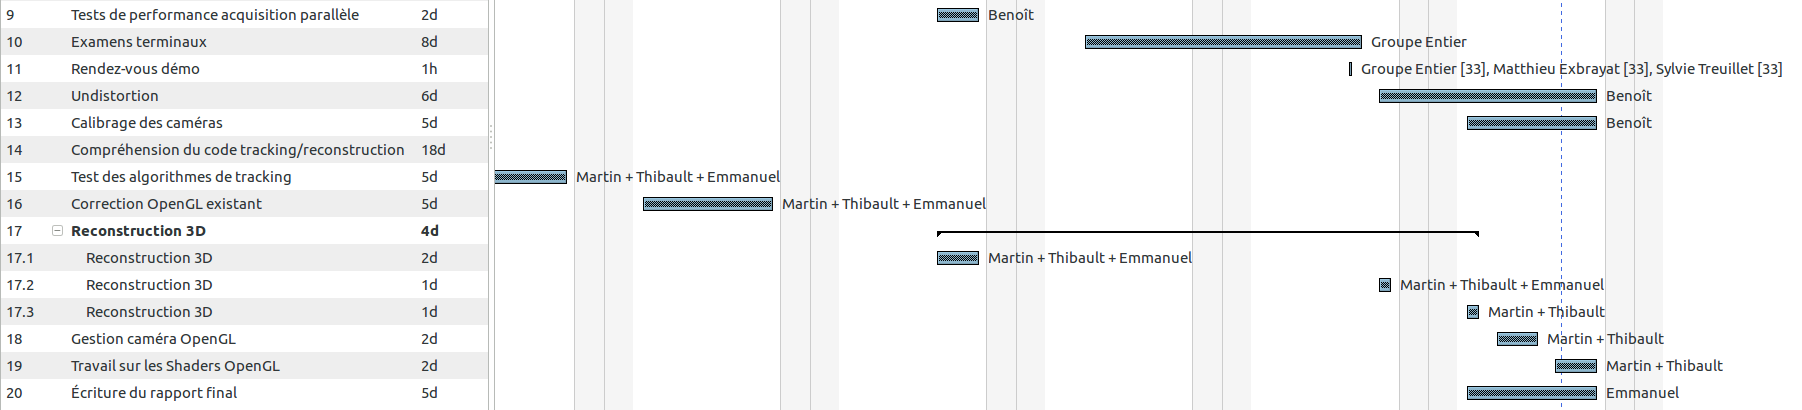
\includegraphics[scale=0.3, angle=90]{Modules/Picture/gantt_final_2}
		\caption{Diagramme de Gantt 2/2}
	\end{center}
\end{figure}

%\begin{figure}
% \begin{minipage}{.5\textwidth}
%  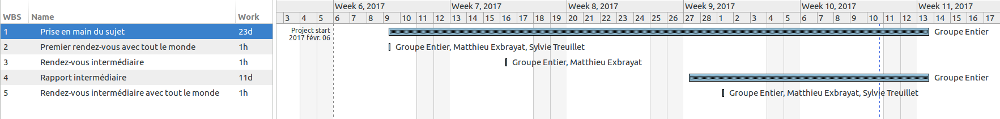
\includegraphics[scale=0.5, angle=90]{Modules/Picture/gantt_final_0}
%  \caption{rr}
% \end{minipage}
% \begin{minipage}{.5\textwidth}
%  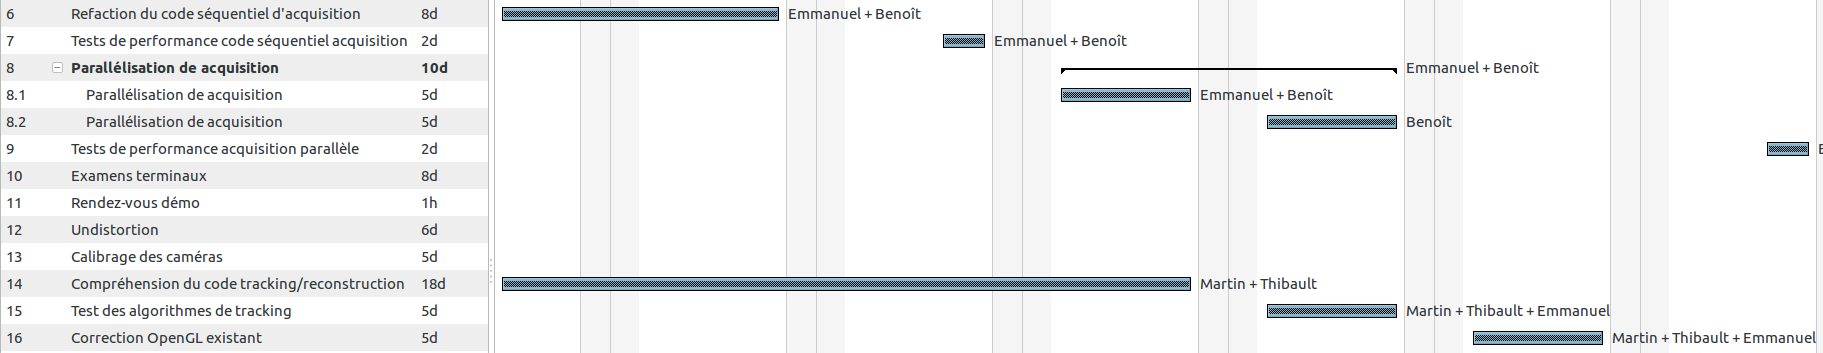
\includegraphics[scale=0.5, angle=90]{Modules/Picture/gantt_final_1}
%  \caption{Diagramme de Gantt}
% \end{minipage}
% \begin{minipage}{.5\textwidth}
%  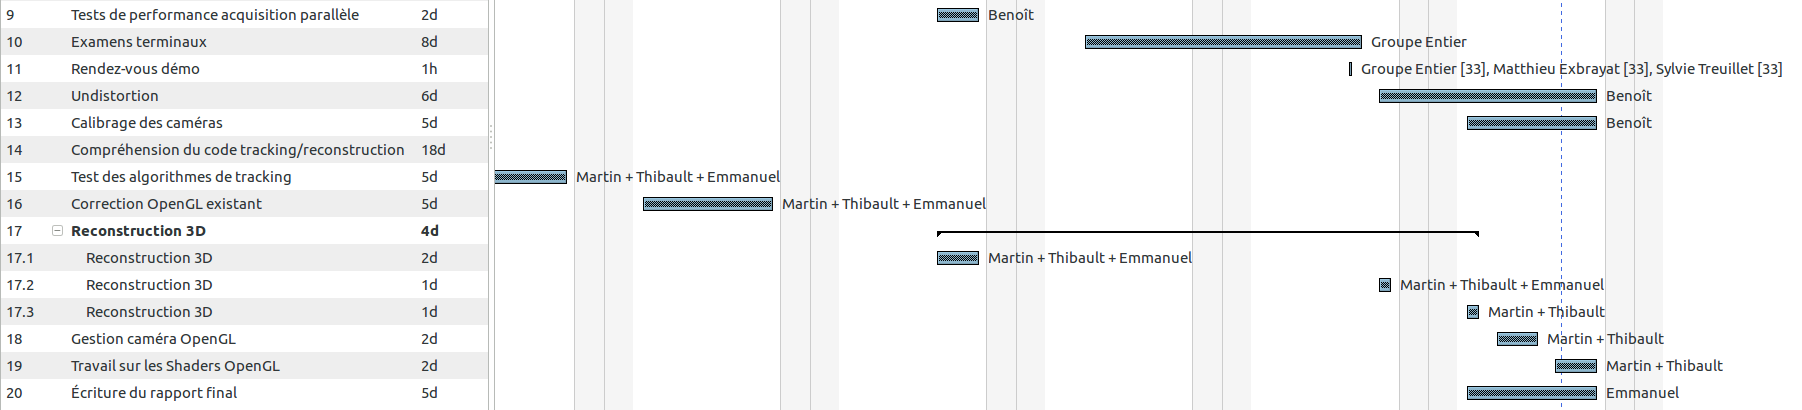
\includegraphics[scale=0.3, angle=90]{Modules/Picture/gantt_final_2}
%  \caption{rr}
% \end{minipage}
%\end{figure}

\newpage

\begin{figure}[!h]
\centering
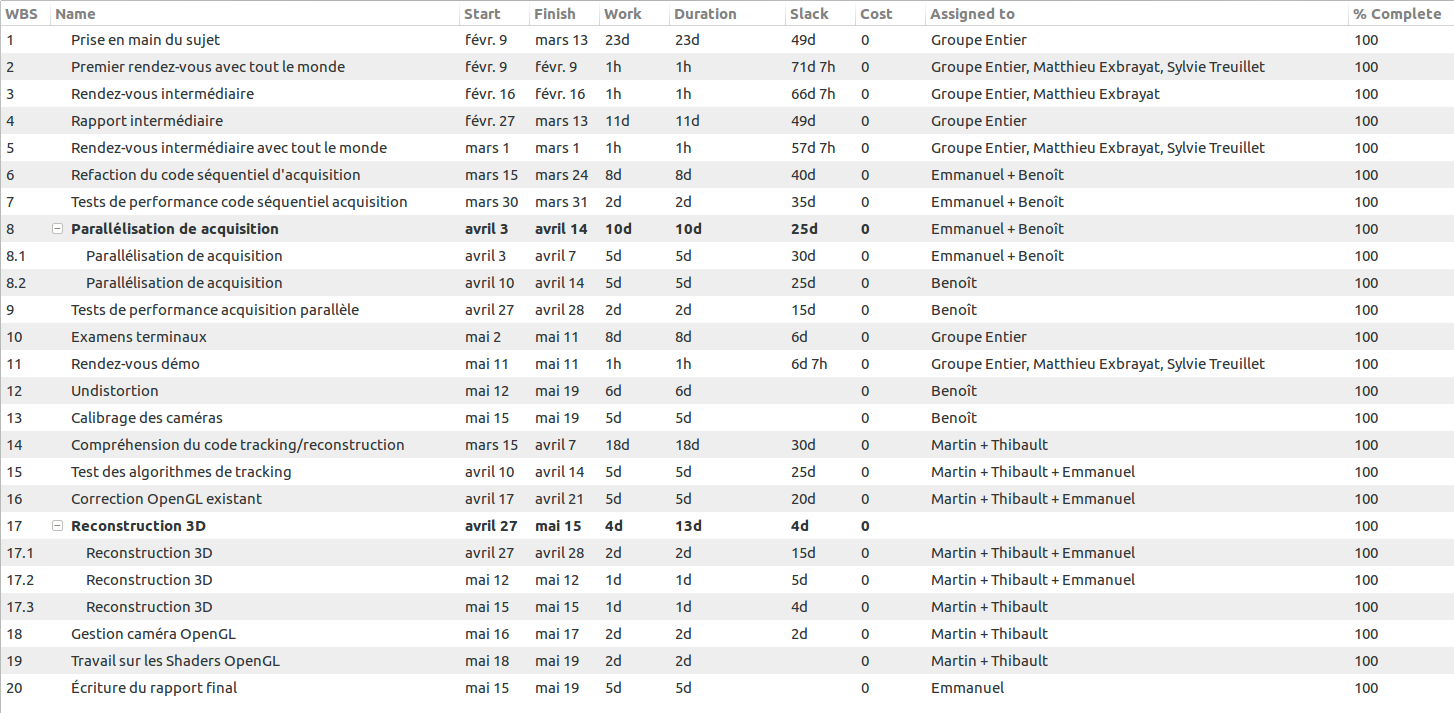
\includegraphics[scale=0.35, angle=90]{Modules/Picture/tableau_gantt_final}
\caption{Diagramme de Gantt - Total}
\label{ganttTableau}
\end{figure}

\clearpage

\newpage



\section{Manuel d'utilisation}

Pour pouvoir lancer et utiliser cette application, différentes bibliothèques doivent être installées sur l'ordinateur. Toutes les manipulations sont décrites pour un environnement Linux (ou Mac), mais peuvent être transposées assez facilement pour Windows.

\subsection{Installation}

\subsubsection{FlyCap}

FlyCap est le framework de PointGrey, le fabricant des deux caméras, permettant de communiquer dans un programme avec les caméras. L'installation est relativement aisée, il suffit d'aller sur le site du constructeur (\url{https://www.ptgrey.com/support/downloads} ) pour télécharger le framework. Il faut alors renseigner le type de caméra (Chameleon3), le modèle (CM3-U3-13S2C-CS) puis le système d'exploitation utilisé. Il faut ensuite sélectionner "Latest FlyCapture2 Full SDK" dans la partie software. Une fois le téléchargement terminé, un README détaille toutes les étapes nécessaires à l'installation, il suffit de les suivre une à une pour avoir FlyCap en état de marche. Pour vérifier si le logiciel s'est bien installé, il est possible de le lancer dans un terminal via la commande \textit{flycap} pour voir la vue d'une des caméras.

\subsubsection{OpenCV}

OpenCV doit être installé également, afin de profiter de son traitement d'image et de ses algorithmes de tracking. Il a été décidé d'utiliser OpenCV 3, car celui-ci contient un module optionnel OpenCV\textunderscore contrib. Ce dernier contient tous les algorithmes de tracking, c'est un extra-module indispensable pour pouvoir exécuter le projet.

Pour installer OpenCV, voici la marche à suivre :

- On se place dans le dossier de travail et on télécharge les dernières versions OpenCV  et d'OpenCV\textunderscore contrib.

\begin{verbatim}
cd ~/<my_working_directory>
git clone https://github.com/opencv/opencv.git
git clone https://github.com/opencv/opencv_contrib.git
\end{verbatim}

- On se place dans le dossier OpenCV téléchargé et on crée un répertoire temporaire pour le build.

\begin{verbatim}
cd ~/opencv
mkdir build
cd build
\end{verbatim}

- On lance la configuration en n'oubliant pas d'inclure l'extra-module. Cette étape peut prendre un certain temps, jusqu'à 1h30 suivant les machines.

\begin{verbatim}
cmake -D CMAKE_BUILD_TYPE=Release
-DOPENCV_EXTRA_MODULES_PATH=*PATH_TO_FOLDER*/opencv_contrib/modules
-D CMAKE_INSTALL_PREFIX=/usr/local ..
\end{verbatim}

- On démarre l'installation. Si on ne possède que quatre coeur, mieux vaut marquer -j4.

\begin{verbatim}
make -j7
\end{verbatim}

- Dans certains cas, il faut rajouter la ligne suivante dans le .bashrc pour indiquer où se trouvent les librairies OpenCV.

\begin{verbatim}
export LD_LIBRARY_PATH=\$LD_LIBRARY_PATH:/usr/local/lib
\end{verbatim}


\subsubsection{OpenGL, glew, glut et glm}

- Il faut commencer par installer OpenGL et Mesa :

\begin{verbatim}
sudo apt-get install cmake xorg-dev libglu1-mesa-dev
\end{verbatim}

- Pour savoir si l'opération s'est bien passée, il faut regarder que les deux fichiers suivants sont bien présents :

\begin{verbatim}
/usr/include/GL
/usr/lib/x86_64-linux-gnu/libGL.so
\end{verbatim}

- A présent, il faut retourner dans le dossier de travail pour installer GLFW. Commencer par télécharger le code source (\url{https://sourceforge.net/
projects/glfw/files/glfw/3.0.4/glfw-3.0.4.zip/download} ), puis exécuter les instructions suivantes :

\begin{verbatim}
cd glfw-3.0.4
rehash
cmake -G "Unix Makefiles"
make
sudo make install
\end{verbatim}

- Les fichiers suivants doivent maintenant être présents :

\begin{verbatim}
/usr/local/include/GLFW
/usr/local/lib/libglfw3.a
\end{verbatim}

Pour installer glew :
Dans synaptic, installer les packages glew-utils, libglew-dev, libglew1.13, libglewwmx1.13

Pour installer glm :
Dans synaptic, installer le package libglm-dev.

\subsection{Utilisation}

Le travail est séparé en deux parties : acquisition et reconstruction, que l'on retrouve dans deux dossiers différents.

\subsubsection{Acquisition}

Un Makefile est fait pour compiler cette partie. Il permet de compiler le code avec les différentes librairies opencv et flycap. Une fois compilé, il suffit de lancer l'exécutable créé pour lancer l'acquisition stéréo.

\subsubsection{Reconstruction}

Cette partie nécessite plus de bibliothèques, à cause de la reconstruction OpenGL. Le mode de fonctionnement est donc légerement différent. Il faut se placer à l'intérieur du répertoire build, et lancer la commande ccmake ../ pour construire dans le dossier parent l'environnement d'exécution. Il faut ensuite faire la commande make pour compiler le programme. Il suffit alors pour lancer l'application de passer en paramètre de l'exécutable les deux vidéos à traiter pour la reconstruction 3D (dans l'ordre : la vidéo gauche puis droite), puis de se laisser guider par les instructions dans le terminal.

Si on a besoin de faire du tracking, on doit décommenter le $\sharp$define OPENCV qui permettra de lancer le tracking sur les deux vidéos. Après lancement du programme, il y a une fenêtre de choix permettant de parcourir la vidéo frame par frame, afin de savoir à laquelle commencer et finir le tracking. Il faut ensuite quitter cette fenêtre en appuyant sur echap, puis revenir sur le terminal et choisir si on enregistre la vidéo et si on veut sélectionner la partie de la vidéo à traiter. Une fenêtre de sélection de la zone d'interêt apparaît, il faut cliquer avec la souris sur l'objet à suivre, puis agrandir la zone à la souris. Celle zone de sélection peut être modifiée autant de fois que nécessaire, et un appui sur la touche espace permet de lancer le tracking.
Il se passe ensuite la même chose pour la seconde vidéo. Il faut bien penser à appuyer sur echap dans les fenêtres OpenCV pour passer aux parties suivantes.

A partir de cela, des fichiers de points sont créés, fichiers qui seront nécessaires pour faire la reconstruction 3D avec OpenGL. Tant que les fichiers de points sont présents dans le dossier de l'exécutable, il suffit de décommenter le $\sharp$define OPENGL pour lancer la reconstruction 3D (le $\sharp$define OPENCV n'est alors plus nécessaire). Une fenêtre OpenGL s'ouvre, on peut déplacer l'objet dans le repère en 3D grâce à la souris et aux touches zqsd.

\newpage

\bibliographystyle{plain}
\nocite{*}
\bibliography{biblio}

 
\end{document}

\grid
